% ==== Document Class & Packages =====
\documentclass[12pt,hidelinks]{article}
	\usepackage[explicit]{titlesec}
	\usepackage{titletoc}
	\usepackage{tocloft}
	\usepackage{charter}
	\usepackage[many]{tcolorbox}
	\usepackage{amsmath}
	\usepackage{graphicx}
	\usepackage{xcolor}
	\usepackage{tikz,lipsum,lmodern}
	\usetikzlibrary{calc}
	\usepackage[english]{babel}
	\usepackage{fancyhdr}
	\usepackage{mathrsfs}
	\usepackage{empheq}
	\usepackage{fourier}% change to lmodern if fourier is no available
	\usepackage{wrapfig}
	\usepackage{fancyref}
	\usepackage{hyperref}
	\usepackage{cleveref}
	\usepackage{listings}
	\usepackage{varwidth}
	\usepackage{longfbox}
	\usepackage{geometry}
	\usepackage{marginnote}

    \usepackage{caption}

%    \usepackage[hyphens]{url}  % allows line breaks at hyphens



	\tcbuselibrary{theorems}
	\tcbuselibrary{breakable, skins}
	\tcbuselibrary{listings, documentation}
	\geometry{
		a4paper,
		left=33mm,
		right=33mm,
		top=20mm}
% ========= Path to images ============
%   - Direct the computer on the path 
% 	  to the folder containg the images
% =====================================
\graphicspath{{./images/}}
% ============= Macros ================
\newcommand{\fillin}{\underline{\hspace{.75in}}{\;}}
\newcommand{\solution}{\textcolor{mordantred19}{Solution:}}
\setlength{\parindent}{0pt}
\addto{\captionsenglish}{\renewcommand*{\contentsname}{Table of Contents}}
\linespread{1.2}
% ======== Footers & Headers ==========
\cfoot{\thepage}
\chead{}\rhead{}\lhead{}
% =====================================
\renewcommand{\thesection}{\arabic{section}}
\newcommand\sectionnumfont{% font specification for the number
	\fontsize{380}{130}\color{myblueii}\selectfont}
\newcommand\sectionnamefont{% font specification for the name "PART"
	\normalfont\color{white}\scshape\small\bfseries }
% ============= Colors ================
% ----- Red -----
\definecolor{mordantred19}{rgb}{0.68, 0.05, 0.0}
% ----- Blue -----
\definecolor{st.patrick\'sblue}{rgb}{0.14, 0.16, 0.48}
\definecolor{teal}{rgb}{0.0, 0.5, 0.5}
\definecolor{beaublue}{rgb}{0.74, 0.83, 0.9}
\definecolor{mybluei}{RGB}{0,173,239}
\definecolor{myblueii}{RGB}{63,200,244}
\definecolor{myblueiii}{RGB}{199,234,253}
% ---- Yellow ----
\definecolor{blond}{rgb}{0.98, 0.94, 0.75}
\definecolor{cream}{rgb}{1.0, 0.99, 0.82}
% ----- Green ------
\definecolor{emerald}{rgb}{0.31, 0.78, 0.47}
\definecolor{darkspringgreen}{rgb}{0.09, 0.45, 0.27}
% ---- White -----
\definecolor{ghostwhite}{rgb}{0.97, 0.97, 1.0}
\definecolor{splashedwhite}{rgb}{1.0, 0.99, 1.0}
% ---- Grey -----
\definecolor{whitesmoke}{rgb}{0.96, 0.96, 0.96}
\definecolor{lightgray}{rgb}{0.92, 0.92, 0.92}
\definecolor{floralwhite}{rgb}{1.0, 0.98, 0.94}
% ========= Part Format ==========
\titleformat{\section}
{\normalfont\huge\filleft}
{}
{20pt}
{\begin{tikzpicture}[remember picture,overlay]
	\fill[myblueiii] 
	(current page.north west) rectangle ([yshift=-13cm]current page.north east);   
\node[
	fill=mybluei,
	text width=2\paperwidth,
	rounded corners=6cm,
	text depth=18cm,
	anchor=center,
	inner sep=0pt] at (current page.north east) (parttop)
	{\thepart};%
\node[
	anchor=south east,
	inner sep=0pt,
	outer sep=0pt] (partnum) at ([xshift=-20pt]parttop.south) 
	{\sectionnumfont\thesection};
\node[
	anchor=south,
	inner sep=0pt] (partname) at ([yshift=2pt]partnum.south)   
	{\sectionnamefont SECTION};
\node[
	anchor=north east,
	align=right,
	inner xsep=0pt] at ([yshift=-0.5cm]partname.east|-partnum.south) 
	{\parbox{.7\textwidth}{\raggedleft#1}};
\end{tikzpicture}%
}
% ========= Hyper Ref ===========
\hypersetup{
	colorlinks,
	linkcolor={red!50!black},
	citecolor={blue!50!black},
	urlcolor={blue!80!black}
}
% ========= Example Boxes =============
\tcbset{
	defstyle/.style={
		fonttitle=\bfseries\upshape, 
		fontupper=\slshape,
		arc=0mm, 
		beamer,
		colback=blue!5!white,
		colframe=blue!75!black},
	theostyle/.style={
		fonttitle=\bfseries\upshape, 
		fontupper=\slshape,
		colback=red!10!white,
		colframe=red!75!black},
	visualstyle/.style={
		height=6.5cm,
		breakable,
		enhanced,
		leftrule=0pt,
		rightrule=0pt,
		bottomrule=0pt,
		outer arc=0pt,
		arc=0pt,
		colframe=mordantred19,
		colback=lightgray,
		attach boxed title to top left,
		boxed title style={
			colback=mordantred19,
			outer arc=0pt,
			arc=0pt,
			top=3pt,
			bottom=3pt,
		},
		fonttitle=\sffamily,},
	discussionstyle/.style={
		height=6.5cm,
		breakable,
		enhanced,
		rightrule=0pt,
		toprule=0pt,
		outer arc=0pt,
		arc=0pt,
		colframe=mordantred19,
		colback=lightgray,
		attach boxed title to top left,
		boxed title style={
			colback=mordantred19,
			outer arc=0pt,
			arc=0pt,
			top=3pt,
			bottom=3pt,
		},
		fonttitle=\sffamily},
	mystyle/.style={
		height=6.5cm,
		breakable,
		enhanced,
		rightrule=0pt,
		leftrule=0pt,
		bottomrule=0pt,
		outer arc=0pt,
		arc=0pt,
		colframe=mordantred19,
		colback=lightgray,
		attach boxed title to top left,
		boxed title style={
			colback=mordantred19,
			outer arc=0pt,
			arc=0pt,
			top=3pt,
			bottom=3pt,
		},
		fonttitle=\sffamily},
	aastyle/.style={
			height=3.5cm,
			enhanced,
			colframe=teal,
			colback=lightgray,
			colbacktitle=floralwhite,
			fonttitle=\bfseries,
			coltitle=black,
		attach boxed title to top center={
	  		yshift=-0.25mm-\tcboxedtitleheight/2,
	   		yshifttext=2mm-\tcboxedtitleheight/2}, 
		boxed title style={boxrule=0.5mm,
			frame code={ \path[tcb fill frame] ([xshift=-4mm]frame.west)
				-- (frame.north west) -- (frame.north east) -- ([xshift=4mm]frame.east)
				-- (frame.south east) -- (frame.south west) -- cycle; },
			interior code={ 
				\path[tcb fill interior] ([xshift=-2mm]interior.west)
				-- (interior.north west) -- (interior.north east)
				-- ([xshift=2mm]interior.east) -- (interior.south east) -- (interior.south west)
				-- cycle;} }
				},
	examstyle/.style={
		height=9.5cm,
		breakable,
		enhanced,
		rightrule=0pt,
		leftrule=0pt,
		bottomrule=0pt,
		outer arc=0pt,
		arc=0pt,
		colframe=mordantred19,
		colback=lightgray,
		attach boxed title to top left,
		boxed title style={
			colback=mordantred19,
			outer arc=0pt,
			arc=0pt,
			top=3pt,
			bottom=3pt,
		},
		fonttitle=\sffamily},
	doc head command={
		interior style={
			fill,
			left color=yellow!20!white, 
			right color=white}},
	doc head environment={
		boxsep=4pt,
		arc=2pt,
		colback=yellow!30!white,
		},
	doclang/environment content=text
}
% ============= Boxes ================
\newtcolorbox[auto counter,number within=section]{example}[1][]{
	mystyle,
	title=Example~\thetcbcounter,
	overlay unbroken and first={
		\path
		let
		\p1=(title.north east),
		\p2=(frame.north east)
		in
		node[anchor=
			west,
			font=\sffamily,
			color=st.patrick\'sblue,
			text width=\x2-\x1] 
		at (title.east) {#1};
	}
}
\newtcolorbox[auto counter,number within=section]{longexample}[1][]{
	examstyle,
	title=Example~\thetcbcounter,
	overlay unbroken and first={
		\path
		let
		\p1=(title.north east),
		\p2=(frame.north east)
		in
		node[anchor=
		west,
		font=\sffamily,
		color=st.patrick\'sblue,
		text width=\x2-\x1] 
		at (title.east) {#1};
	}
}
\newtcolorbox[auto counter,number within=section]{example2}[1][]{
	aastyle,
	title=Example~\thetcbcounter,{}
}
\newtcolorbox[auto counter,number within=section]{discussion}[1][]{
	discussionstyle,
	title=Discussion~\thetcbcounter,
	overlay unbroken and first={
		\path
		let
		\p1=(title.north east),
		\p2=(frame.north east)
		in
		node[anchor=
		west,
		font=\sffamily,
		color=st.patrick\'sblue,
		text width=\x2-\x1] 
		at (title.east) {#1};
	}
}
\newtcolorbox[auto counter,number within=section]{visualization}[1][]{
	visualstyle,
	title=Visualization~\thetcbcounter,
	overlay unbroken and first={
		\path
		let
		\p1=(title.north east),
		\p2=(frame.north east)
		in
		node[anchor=
		west,
		font=\sffamily,
		color=st.patrick\'sblue,
		text width=\x2-\x1] 
		at (title.east) {#1};
	}
}


% --------- Theorems ---------
\newtcbtheorem[number within=subsection,crefname={definition}{definitions}]%
	{Definition}{Definition}{defstyle}{def}%
\newtcbtheorem[use counter from=Definition,crefname={theorem}{theorems}]%
	{Theorem}{Theorem}{theostyle}{theo}
	%
\newtcbtheorem[use counter from=Definition]{theo}{Theorem}%
{
	theorem style=plain,
	enhanced,
	colframe=blue!50!black,
	colback=yellow!20!white,
	coltitle=red!50!black,
	fonttitle=\upshape\bfseries,
	fontupper=\itshape,
	drop fuzzy shadow=blue!50!black!50!white,
	boxrule=0.4pt}{theo}
\newtcbtheorem[use counter from=Definition]{DashedDefinition}{Definition}%
 {
 	enhanced,
 	frame empty,
 	interior empty,
 	colframe=darkspringgreen!50!white,
	coltitle=darkspringgreen!50!black,
	fonttitle=\bfseries,
	colbacktitle=darkspringgreen!15!white,
	borderline={0.5mm}{0mm}{darkspringgreen!15!white},
	borderline={0.5mm}{0mm}{darkspringgreen!50!white,dashed},
	attach boxed title to top center={yshift=-2mm},
	boxed title style={boxrule=0.4pt},
	varwidth boxed title}{theo}
%%%%%%%%%%%%%%%%%%%%%%%%%%%%%%%%%%%%%%%%
\newtcblisting[auto counter,number within=section]{disexam}{
	skin=bicolor,
	colback=white!30!beaublue,
	colbacklower=white,
	colframe=black,
	before skip=\medskipamount,
	after skip=\medskipamount,
	fontlower=\footnotesize,
	listing options={style=tcblatex,texcsstyle=*\color{red!70!black}},}
%%%%%%%%%%%%%%%%%%%%%%%%%%%%%%%%%%%%%%%

% ===== Code block style for command-line =====
\lstdefinestyle{bashstyle}{
    backgroundcolor=\color{gray!10},   % light gray background
    basicstyle=\ttfamily\footnotesize,        % typewriter font
    breaklines=true,                   % automatic line breaks
    frame=single,                      % box around code
    showstringspaces=false,
    numbers=left,                      % optional line numbers
    numberstyle=\tiny\color{gray},     % style for line numbers
    keywordstyle=\color{blue},         % optional color for keywords
}



%%%%%%%%%%%%%%%%%%%%%%%%%%%%%%%%%%%%%%%%%%%%%%%%%%%%%%%%%%%%%%%%%%%%%%%%%%%%%%%%%%%%%%%%%%%%%%%%%%%%%%%%%%%%%%%%%%%%%
\begin{document}
\begin{titlepage}
	\centering % Center everything on the title page
	\scshape % Use small caps for all text on the title page
	\vspace*{1.5\baselineskip} % White space at the top of the page
% ===================
%	Title Section 	
% ===================

	\rule{13cm}{1.6pt}\vspace*{-\baselineskip}\vspace*{2pt} % Thick horizontal rule
	\rule{13cm}{0.4pt} % Thin horizontal rule
	
		\vspace{0.75\baselineskip} % Whitespace above the title
% ========== Title ===============	
	{	\Huge Manual\\
			\vspace{4mm}
		Driver Monitoring System \\	}
% ======================================
		\vspace{0.75\baselineskip} % Whitespace below the title
	\rule{13cm}{0.4pt}\vspace*{-\baselineskip}\vspace{3.2pt} % Thin horizontal rule
	\rule{13cm}{1.6pt} % Thick horizontal rule
	
		\vspace{1.75\baselineskip} % Whitespace after the title block
% =================
%	Information	
% =================
	{\large Produced by: Khongmeng Kormoua \\
		\vspace*{1.2\baselineskip}
	korm4202@stthomas.edu} \\
	\vfill
If you come across any problems, see section \ref{sec:issue} for possible\\ \vspace{1mm}
solutions or contact me at \url{korm4202@stthomas.edu}
\end{titlepage}
%%%%%%%%%%%%%%%%%%%%%%%%%%%%%%%%%%%%%%%%%%%%%%%%%%%%%%%%%%%%%%%%%%%%%%%%%%%%%%%%%%%%%%%%%%%%%%%%%%%%%%%%%%%%%%%%%%%%%%
\tableofcontents
\vfill
\small{\noindent \textbf{About This File} \vspace{-3mm}\\
\noindent \rule{3.3cm}{0.5pt} \\
This file was created for the benefit of all researchers as a guideline on reproducing and understanding problem encountered on the project.}
\newpage
\newgeometry{
	left=29mm, 
	right=29mm, 
	top=20mm, 
	bottom=15mm}
%%%%%%%%%%%%%%%%%%%%%%%%%%%%%%%%%%%%%%%%%%%%%%%%%%%%%%%%%%%%%%%%%%%%%%%%%%%%%%%%%%%%%%%%%%%%%%%%%%%%%%%%%%%%%%%%%%%%%%
\section{Hardware Setup}
\vspace{10.5cm}
	\textbf{\emph{Remember that, it is always safer to insert/remove hardware while the system is turned off. Otherwise, it may damage the system.}}

    \subsection{Hardware Lists}
    \label{subsec:hardware_list}
			Hardwares used in this project will be listed in this section with link to them as of now (Sep 25, 2025). To interface with the hardware, a keyboard, mouse and monitor with display port is used in this project. Other option such as Virtual Network Computing (VNC)\footnote{\url{https://www.realvnc.com/}} is popular and commonly used in community.

            \sloppy
            \begin{itemize}
                \item Developement board: Jetson Orin Nano Developer Kit - 8GB ({\footnotesize \url{https://www.nvidia.com/en-us/autonomous-machines/embedded-systems/jetson-orin/nano-super-developer-kit/}}).
                \\
                \begin{center}
                    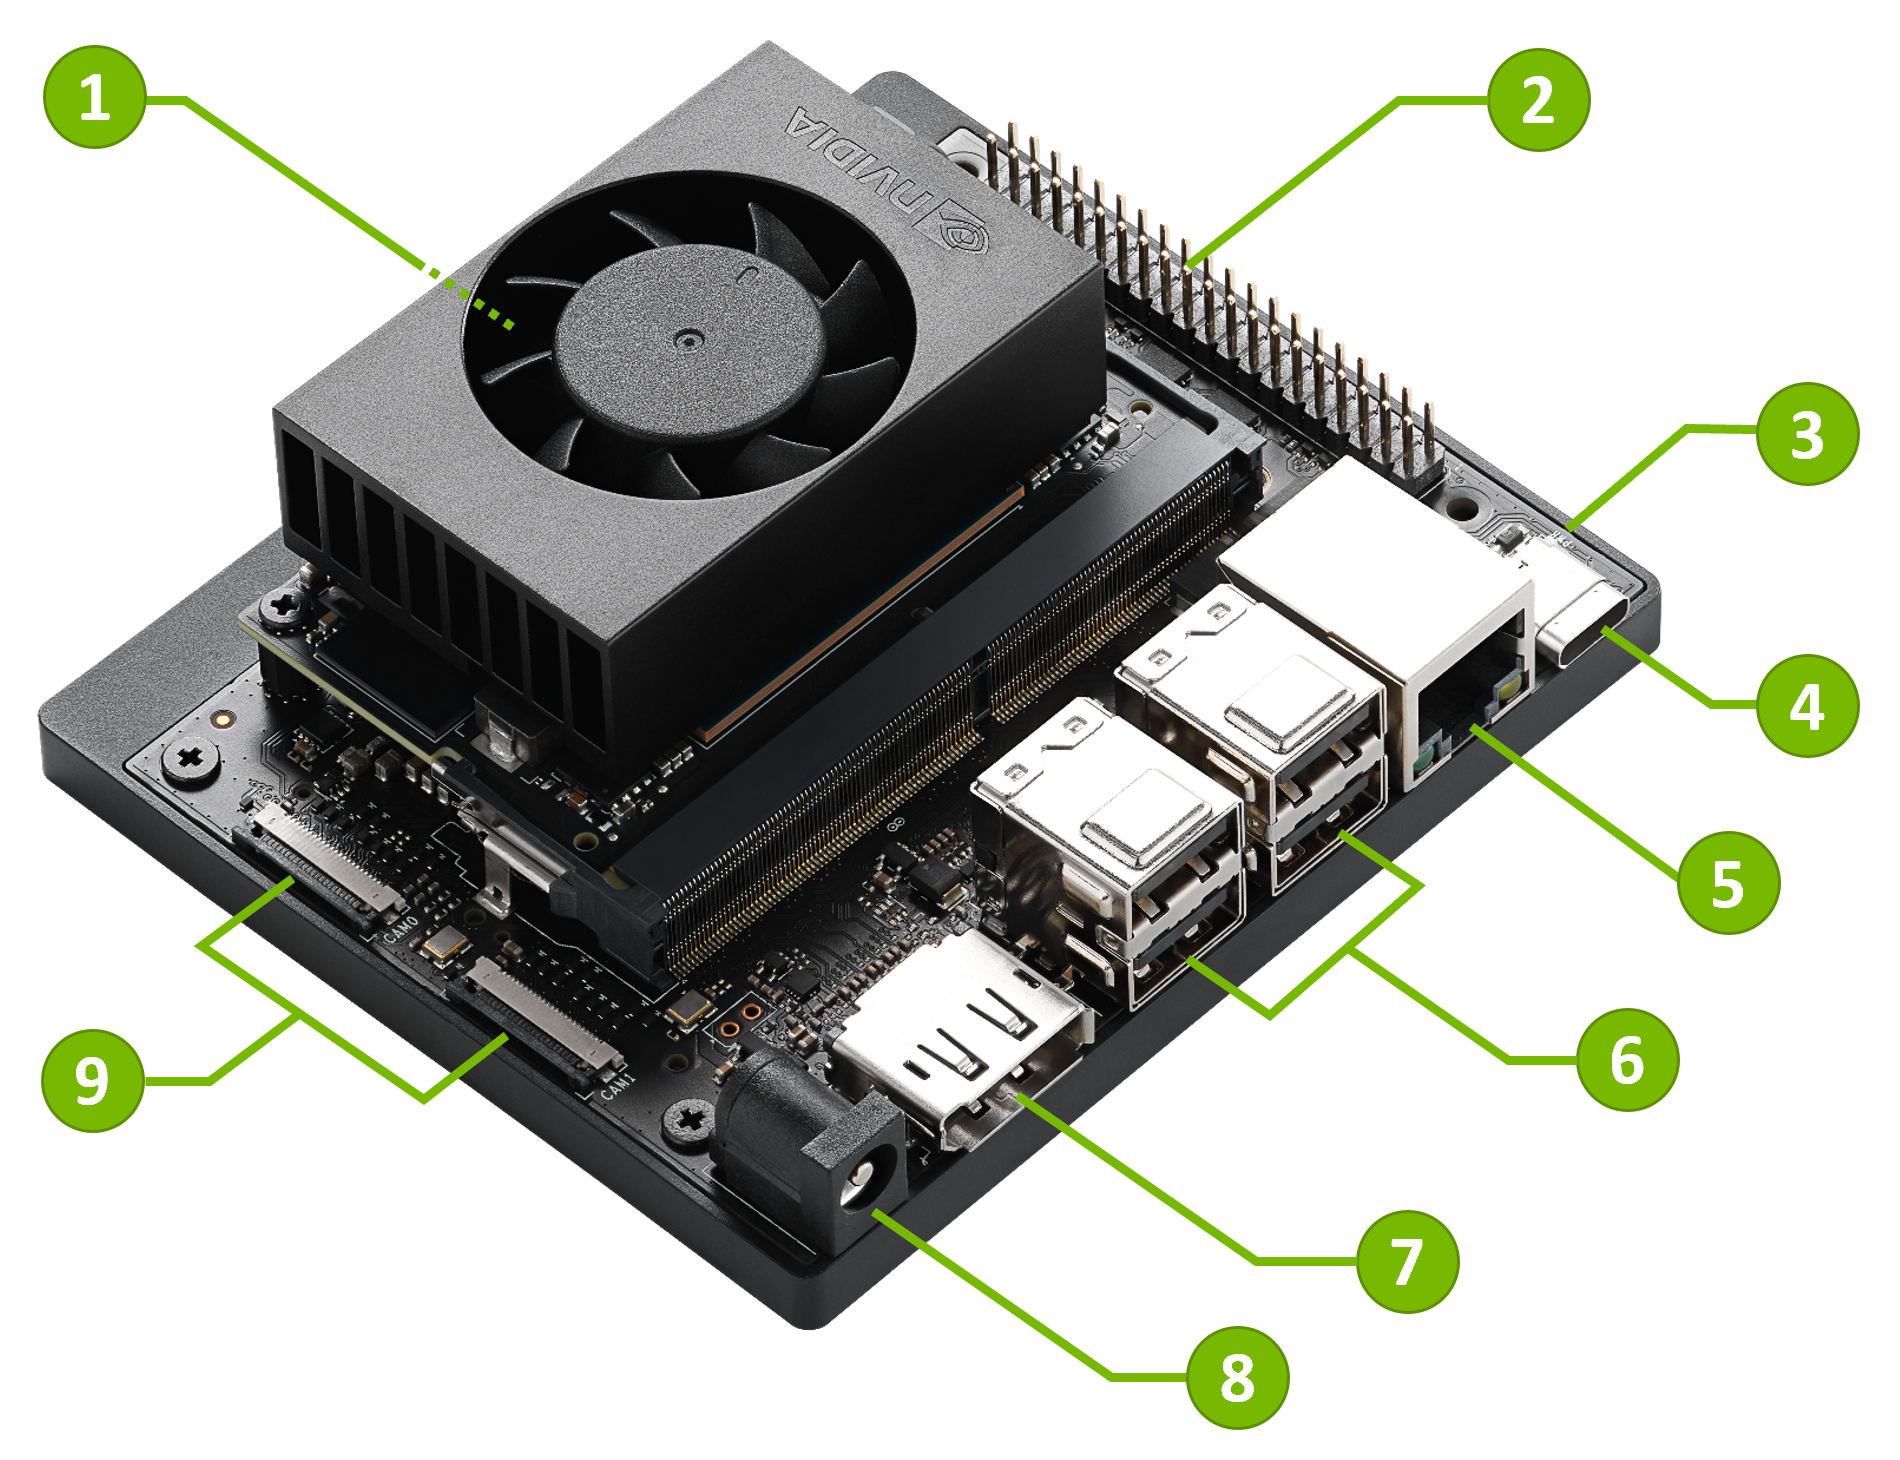
\includegraphics[width=0.4\textwidth]{pics/jetson-orin-nano-front_numbered.png}
                    \captionof{figure}{Jetson Orin Nano}
                    \label{fig:jetson}
                \end{center}
                

                \item Camera Module: Arducam Day and Night Vision IMX477 HQ Camera for Jetson Orin NX, 12MP Automatic IR-Cut Switching for All-Day Image ({\footnotesize \url{https://a.co/d/03FuGEy}}). This camera is used becaues, it has daytime and night time image capturing capability at 1080P at 60Hz in reasonable price. Other options in similar specs are fairly expensive for research propose or prototype v1.
                \\
                \begin{center}
                    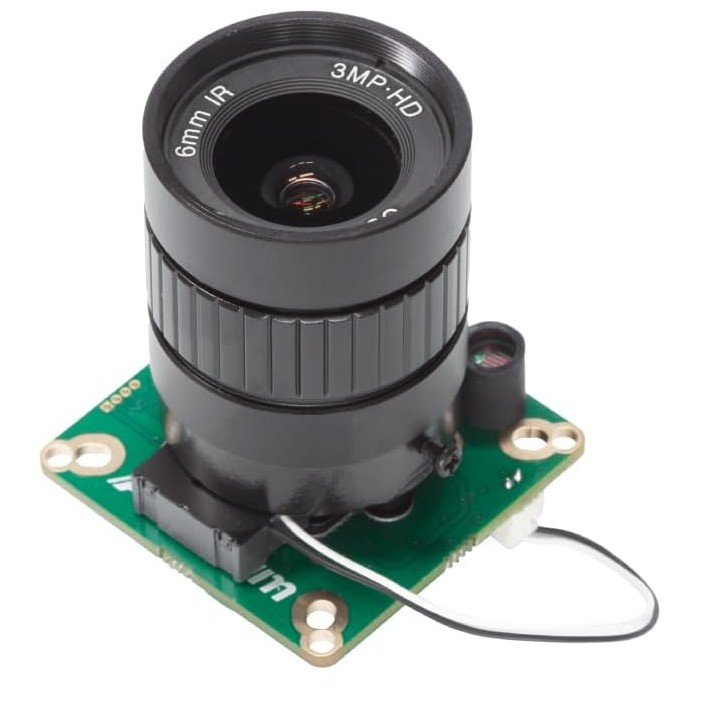
\includegraphics[width=0.3\textwidth]{pics/ArduCam_camera.jpg}
                    \captionof{figure}{Arducam}
                    \label{fig:arducam}
                \end{center}
                

                \item Storage: Samsung 990 Evo Plus 1TB ({\footnotesize \url{https://www.samsung.com/us/computing/memory-storage/solid-state-drives/990-evo-plus-gen5-pcie-nvmetm-ssd-1tb-mz-v9s1t0b-am/}}). Make sure that the SSD is NVMe type not SATA as SATA SSD is not compatible with Jetson Orin Nano.
                \\

                \begin{center}
                    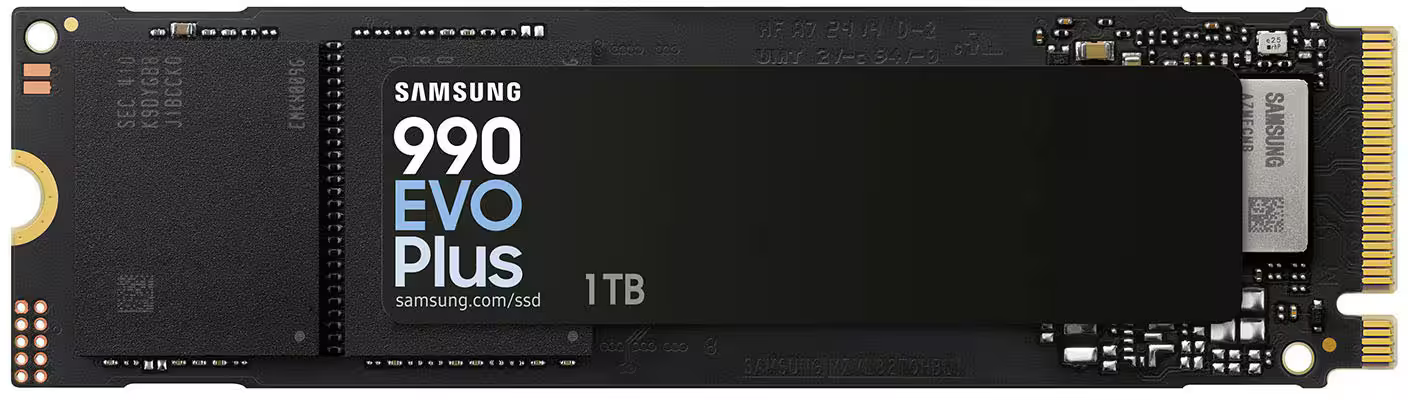
\includegraphics[width=0.4\textwidth]{pics/samsung_ssd.png}
                    \captionof{figure}{SSD}
                    \label{fig:ssd}
                \end{center}

                \item Keyboard.
                \item Mouse.
                \item Monitor: Monitor with display port or adaptor since Jetson Orin Nano only has disply port available.
            \end{itemize}


            
	\subsection{Installing Solid State Drive (SSD)}
    \label{subsec:jetson_back}
    
			On the back of Jetson Orin Nano, ther are three slots as shown in Figure  \ref{fig:jetson_back}. A Wi-Fi and Bluetooth card should be included and installed at slot 12 already, if not it is needed and will be added to hardware list. A SSD will need to be installed at slot 10.

    \begin{figure}[ht] % h = here
        \centering
        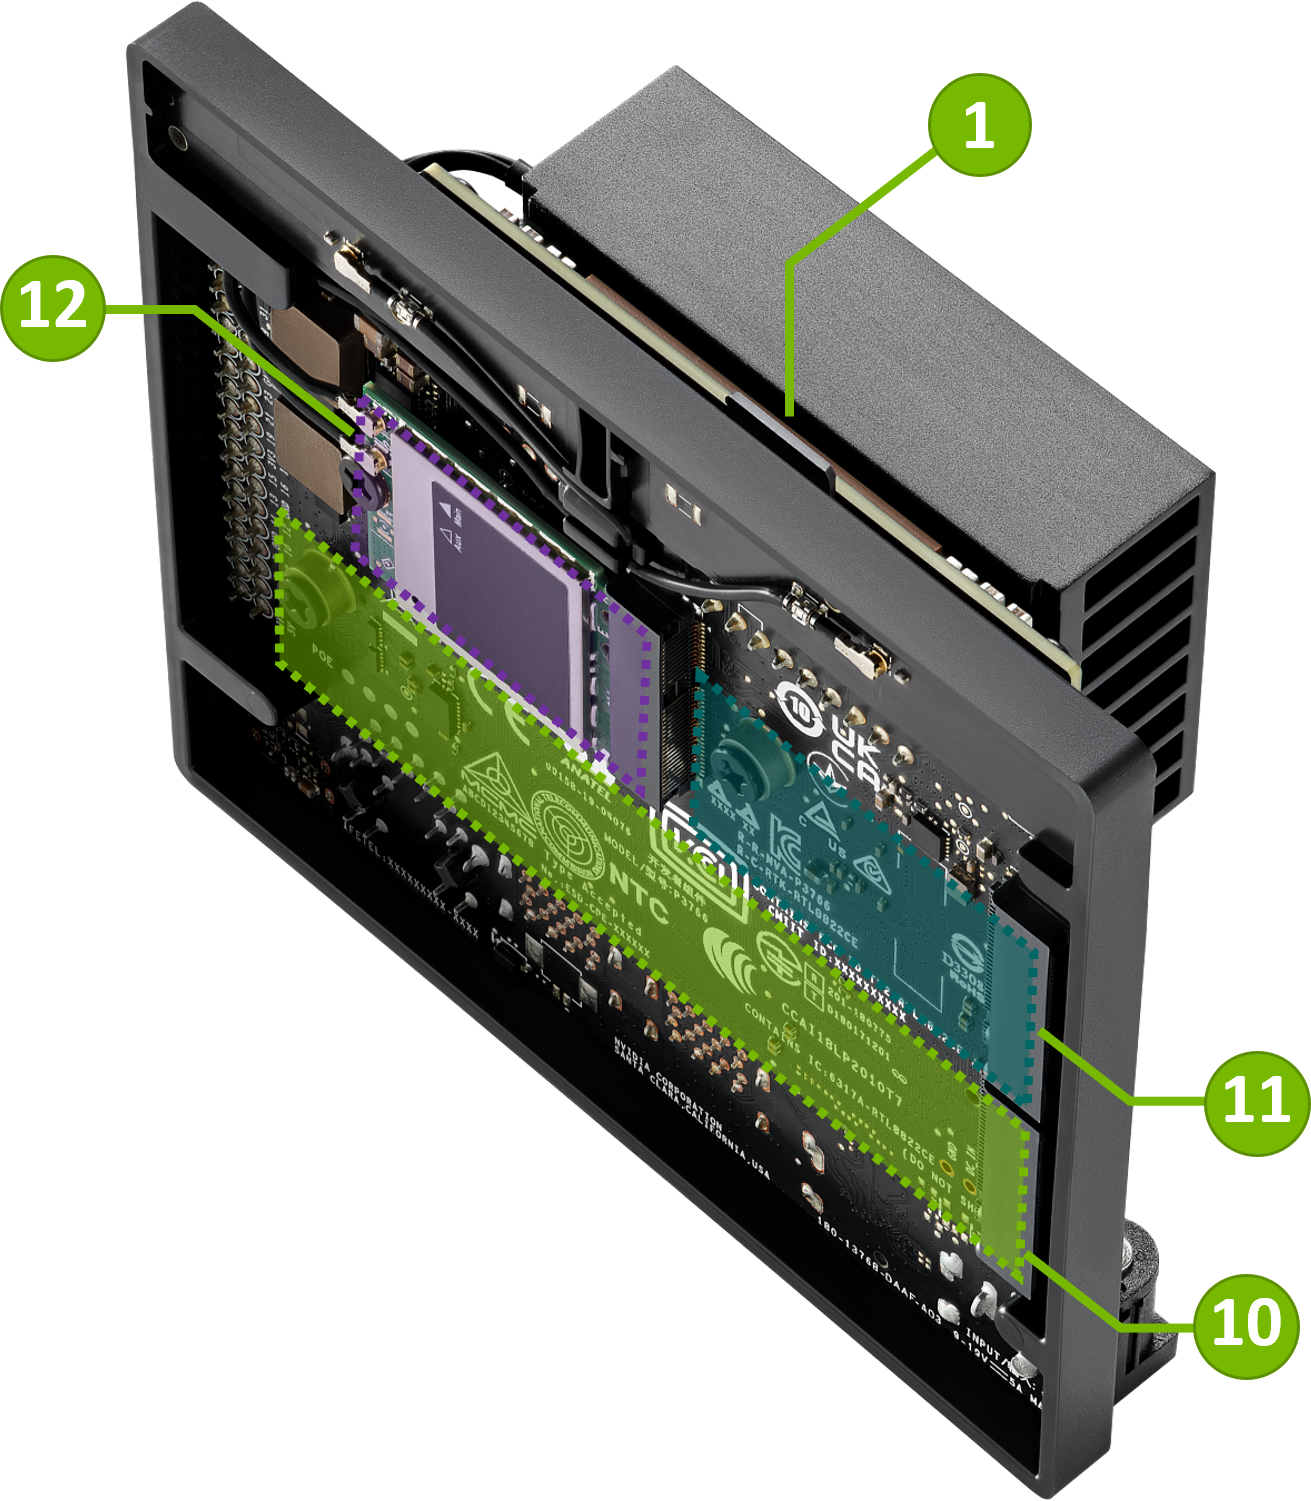
\includegraphics[width=0.5\textwidth]{pics/jetson_orin_nano_back_numbered.png}
        \caption{Jetson Orin Nano - Back.}
        \label{fig:jetson_back}
    \end{figure}


    \subsection{Flashing and Installing Jetpack Operating System}
    \label{subsec:flashing_jetpack}

        \subsubsection{Flashing SSD}
        \label{subsubsec:flashing}

        To start the flashing process, first The Jetson Orin Nano need to be in recovery mode. To do so, use a jumper wire to connect \textbf{\emph{GND}} pin and \textbf{\emph{FC REC}} pin as shown in Figure \ref{fig:jetson_recovery}. 

        \begin{figure}[ht] % h = here
            \centering
            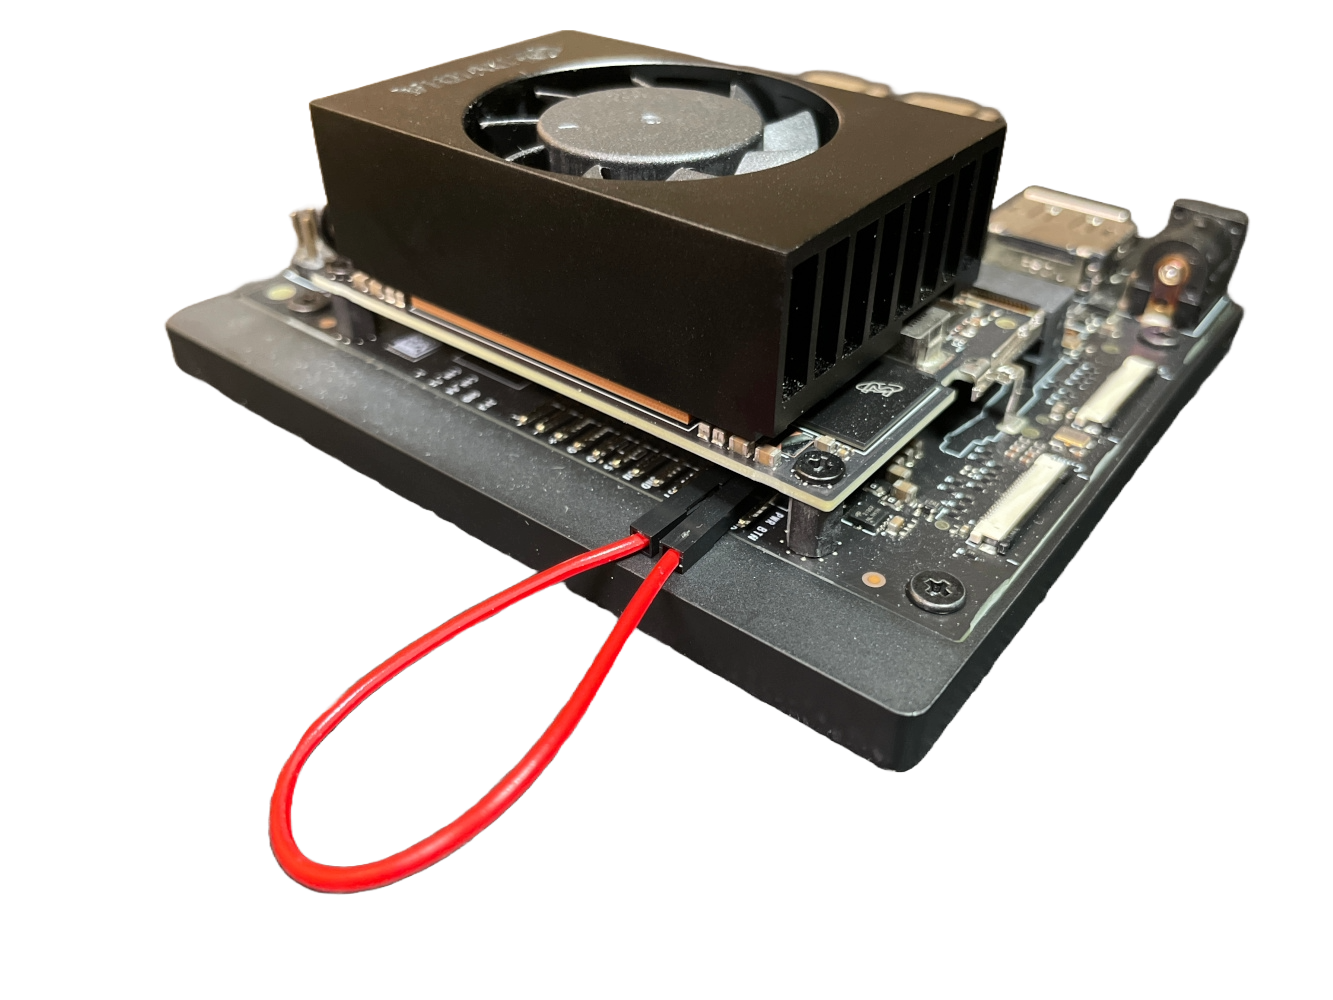
\includegraphics[width=0.5\textwidth]{pics/orin_nano_recovery_mode.png}
            \caption{Jetson Orin Nano - Recovery Mode}
            \label{fig:jetson_recovery}
        \end{figure}


        Then connect keyboard, mouse, monitor, USB cable which will be connected to another PC to flash Jetson Orin Nano as shown in Figure \ref{fig:setup_flashing}. Note that in the figure power cable is connected but, at this step no need to connect power cable yet. power cable will be connected to Jetson Orin Nano once SDK manager is open in step \ref{}.


         \begin{figure}[ht] % h = here
            \centering
            \setlength{\fboxsep}{0pt}
            \setlength{\fboxrule}{1pt}
            \fbox{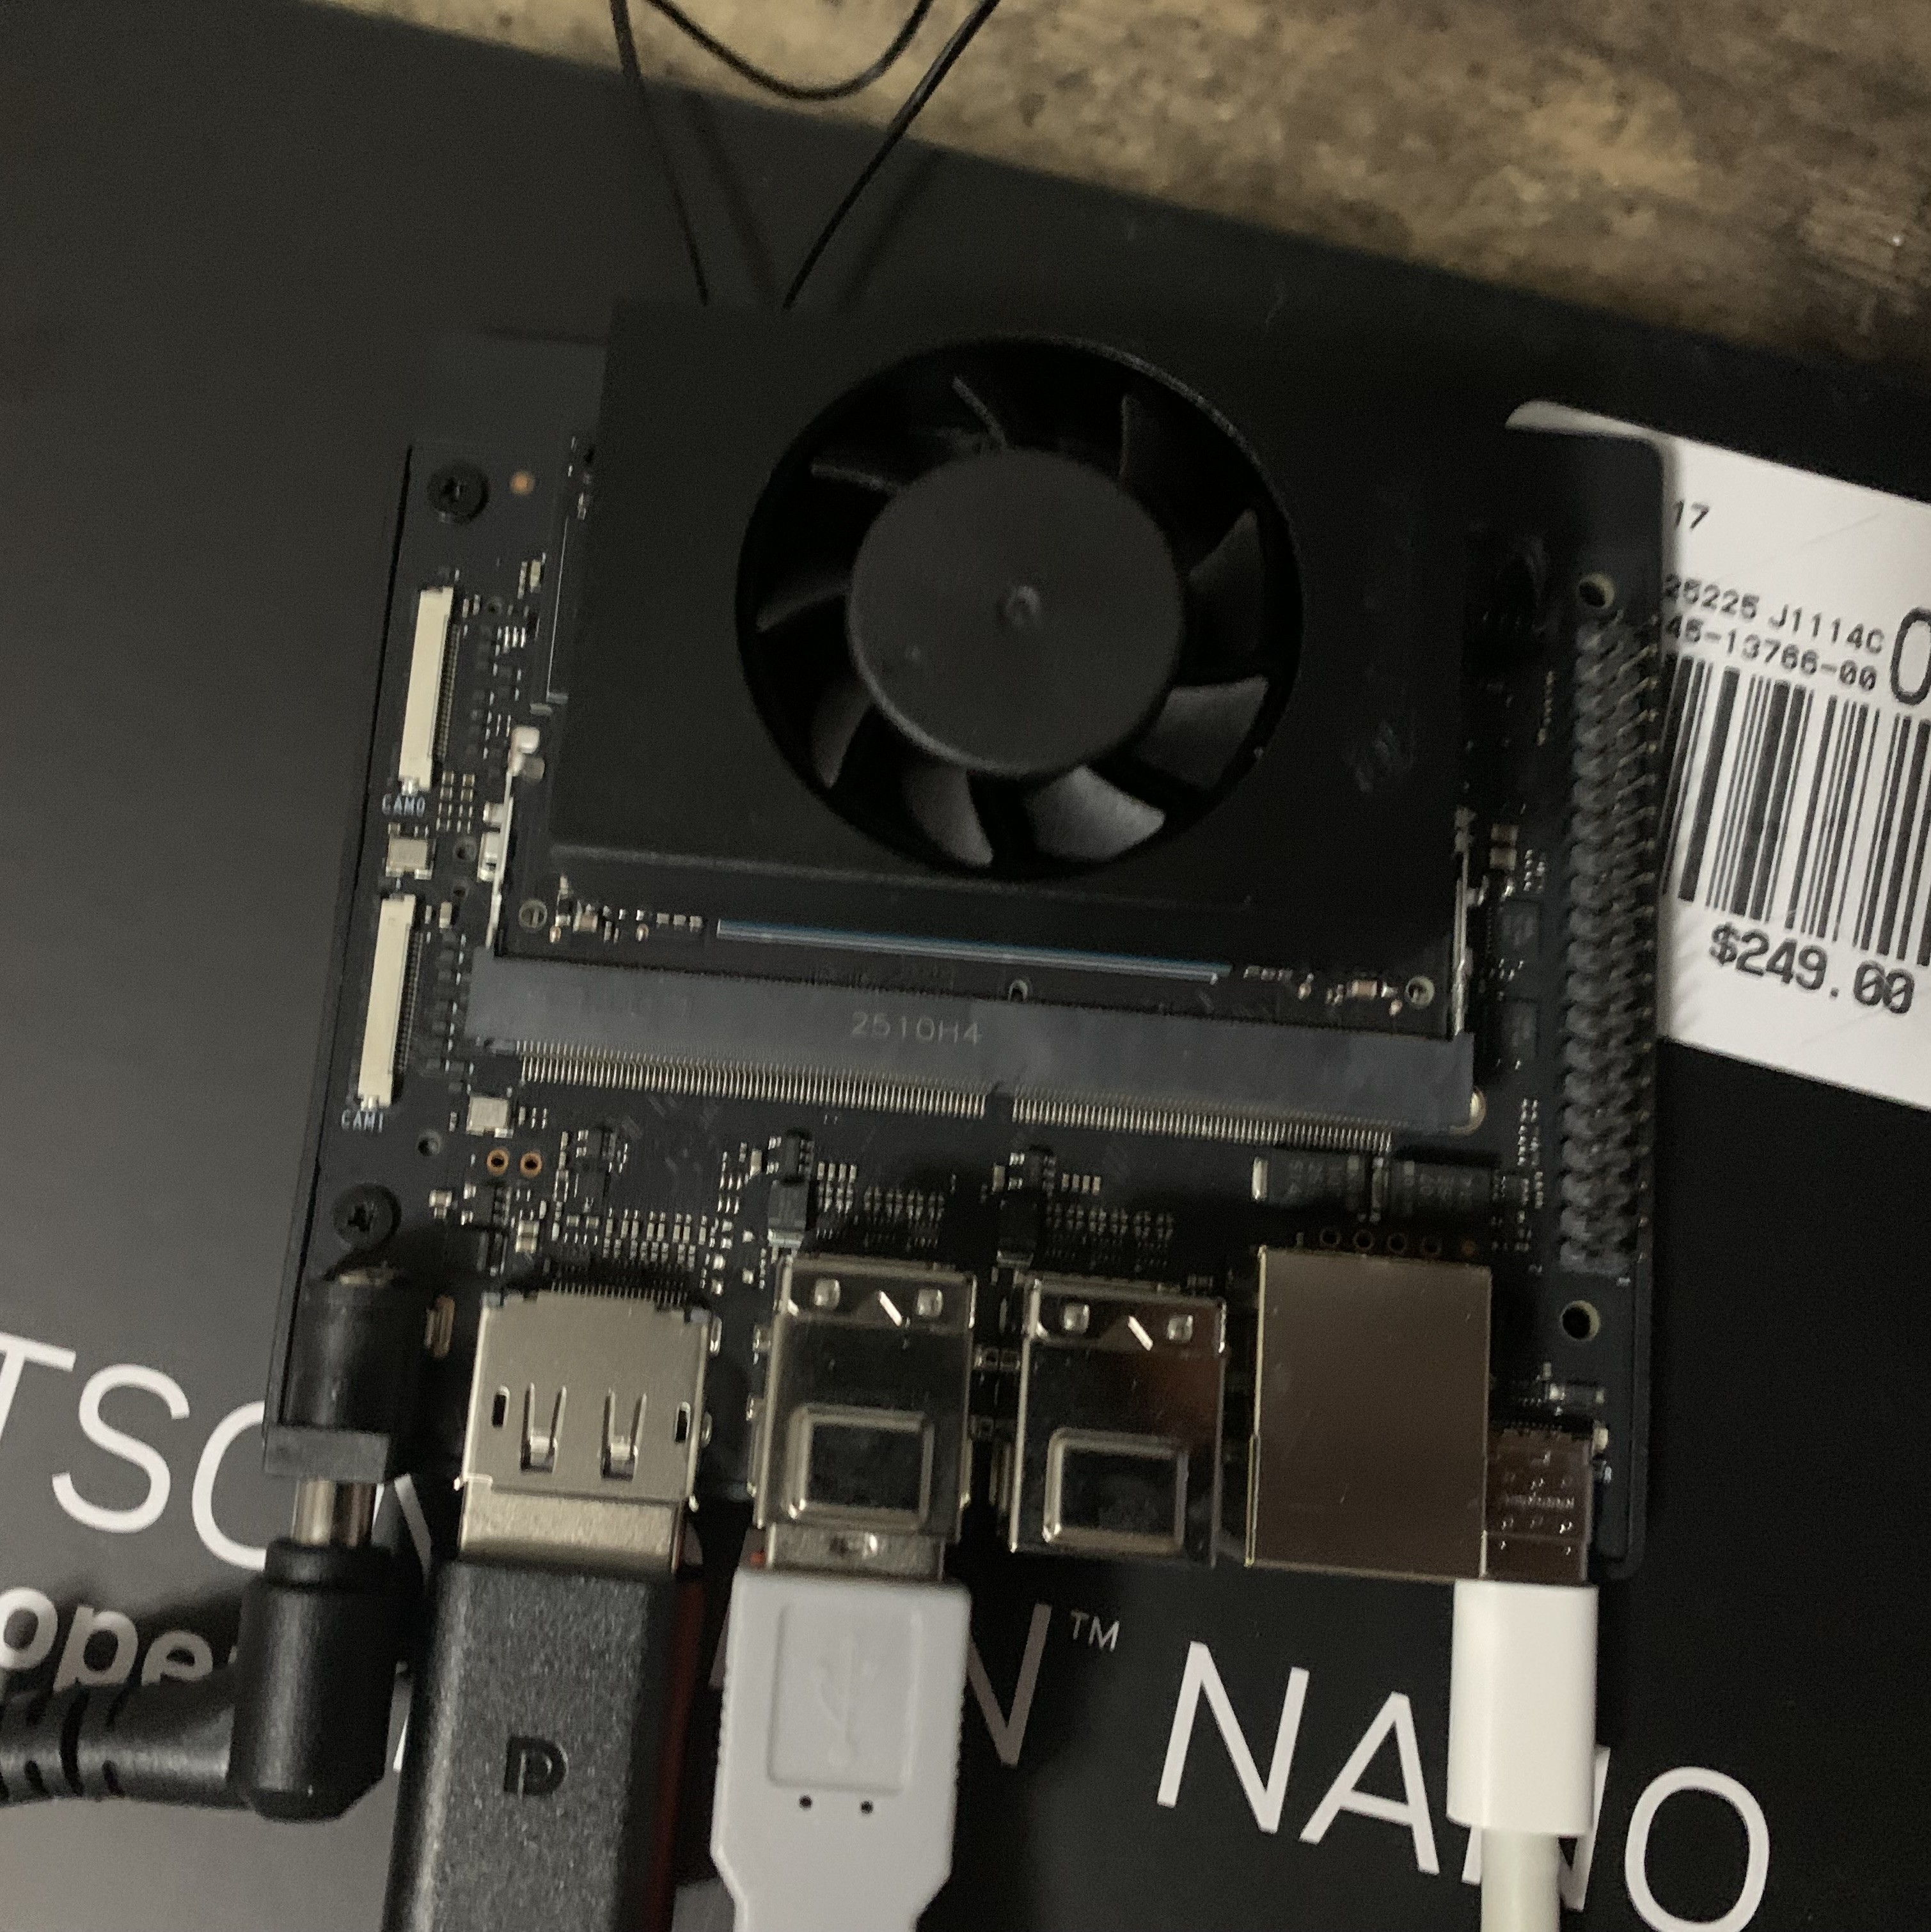
\includegraphics[width=0.5\textwidth]{pics/flashing-recovery-mode.jpg}}
            \caption{Hardware connection for flashing.}
            \label{fig:setup_flashing}
        \end{figure}

        \vspace{3mm}

        After have all hardware connection ready. Ubuntu 22.04.5 LTS version is used on PC to flash the SSD of Jetson Orin Nano. In order to have Ubuntu in Windows system, a VMware Workstation Pro 17.6.4 is used, an Ubuntu is then installed on Virtual Machine (VM). After installing VMware on Windows PC, the installation of Ubuntu on VMware can be done following this tutorial ({\footnotesize \url{https://www.youtube.com/watch?v=SgfrHKg81Qc}}). 

        \vspace{3mm}
        
        When Ubuntu 22.04.5 LTS is ready we can start procedure of flashing and installing Jetpack on Jetson Orin Nano. The whole process can be done following this tutorial ({\footnotesize \url{https://www.youtube.com/watch?v=BaRdpSXU6EM}}). 

        \vspace{3mm}
        
        Note that in this tutorial, it use an older version of SDK manager, version 2.2.0; which required a IP address of Jetson Orin Nano after successfully flashing. But in later version 2.3.0; it is possible to install Jetpack package after flashing SSD via USB without IP address needed. 

        \vspace{3mm}

        Another note is that in the tutorial an ethernet cable is connected to access to internet. In this work however, to access internet only Wi-Fi is used. This will be done after finish flashing the SSD. It is necessary to disconnect the jumper wire to exit from reconvery mode, login into Jetson Orin Nano, connect to Wi-Fi, make sure that Jetson Orin Nano has access to Internet before proceeding to install Jetpack Package.

        \vspace{3mm}

        After successfully installed and boot up Jetpack, browser like Chromium and Firefox is not working. Proceed to section \ref{subsec:issue_chromium_firefox} for detail and solution.

        

    \subsection{Installing Camera}
    \label{subsec:install_camera}

        \subsubsection{Connecting Camera into Jetson Orin Nano}
        \label{subsubsec:connect_camera}

        Both a camera and Jetson Orin Nano have a CSI port that connected by 22 pins (or 24 pins) FFC. So using the cable comes with camerea, they both can be connected. The CSI port has a black lock that need to be pull out first before inserting a cable inside. \textbf{\emph{Make sure that the pin side goes in opposite direction from the black lock.}}. Make sure that the cable is inserted all the way into the port before pushing the black lock back in firmly. After connecting a camera, the first version of hardware prototype connection is done as shown in Figure \ref{fig:hardware_setup_v1}. Where a camera is connected to CAM0, monitor is connected to display port, mouse and keyboard are connected to USB port using a wireless receiver of the mouse and keyboard, and power cable is connected to power port.

        \begin{figure}[ht] % h = here
            \centering
            \setlength{\fboxsep}{0pt}
            \setlength{\fboxrule}{1pt}
            \fbox{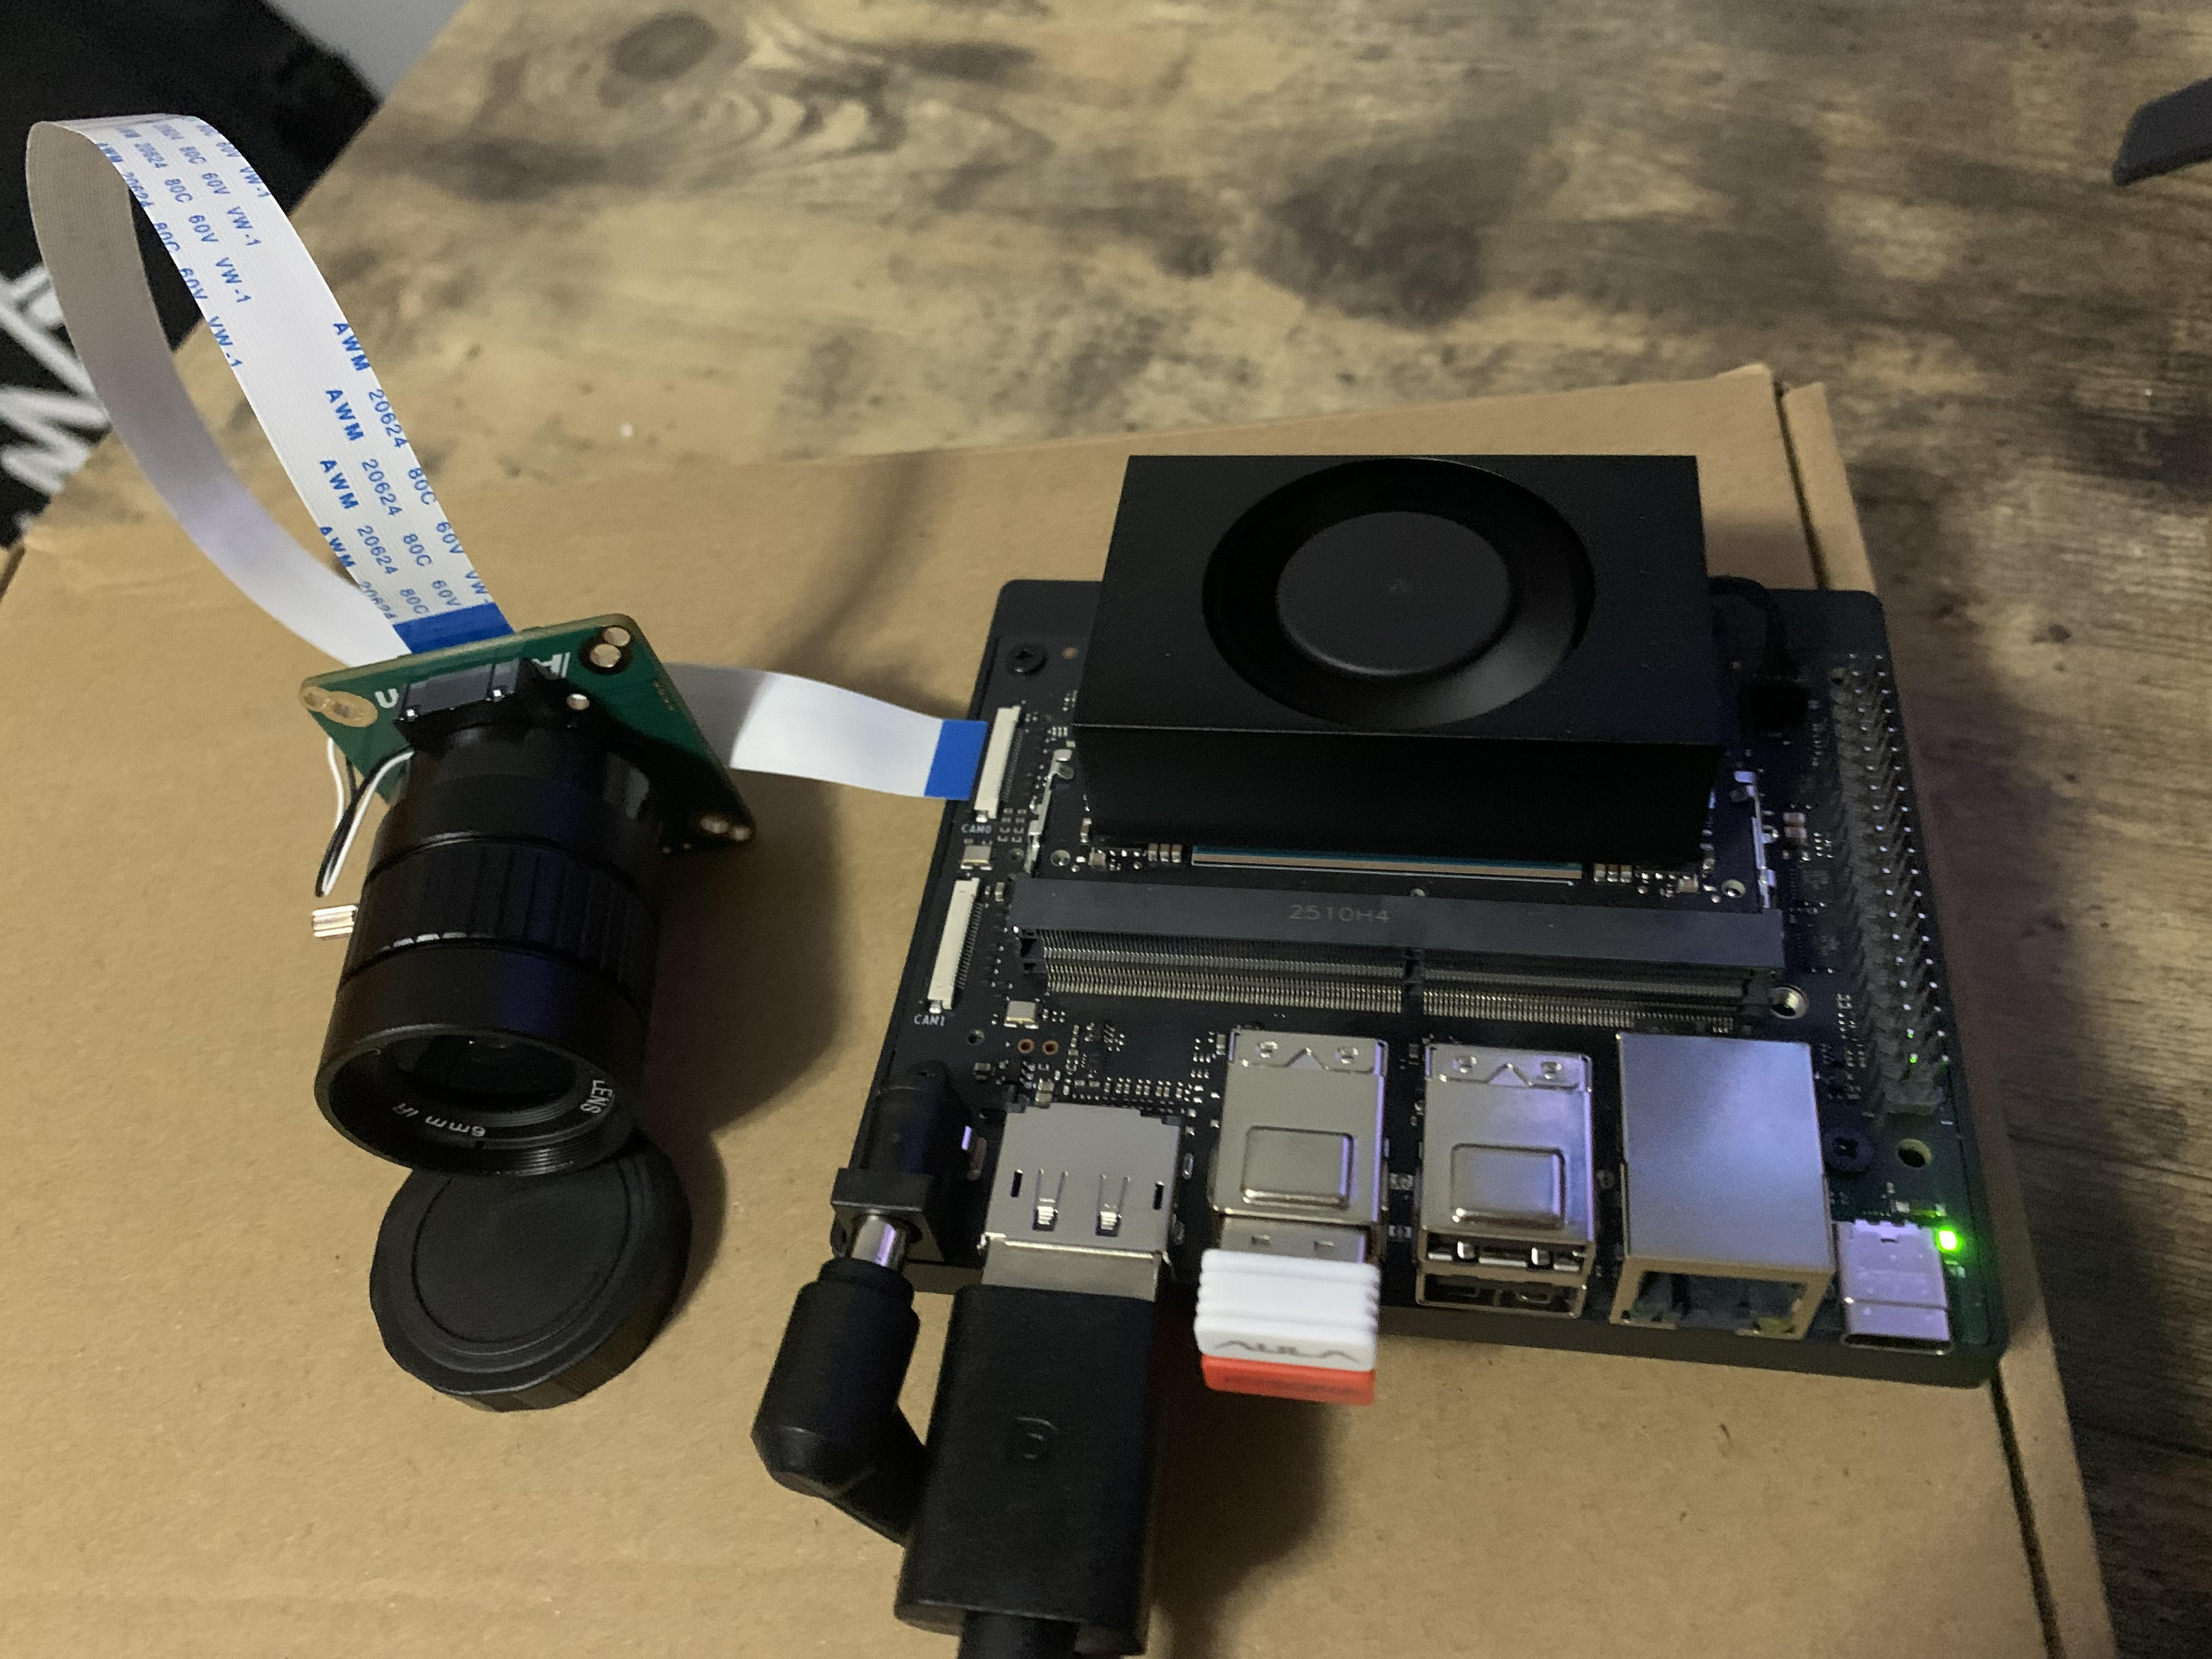
\includegraphics[width=0.7\textwidth]{pics/Hardware_setup_v1.jpg}}
            \caption{Hardware setup V1}
            \label{fig:hardware_setup_v1}
        \end{figure}

        \subsubsection{Software setup for Camera (IMX477)}
        \label{subsubsec:software_setup_imx477}


        After connected a camera to Jetson Orin Nano, the app \textbf{\emph{Cheese}} did not recognize the camera. A simple script from github {\footnotesize \url{https://github.com/JetsonHacksNano/CSI-Camera.git}} to test CSI camera is used. After cloning the repo into local working machine, go inside the repository and use simple command to try a camera.

        \vspace{2mm}

        \begin{lstlisting}[style=bashstyle]
$ python3 simple_camera.py
        \end{lstlisting}

        However, initially this would give an error about cannot detect a camera. Proceed to section \ref{subsec:camera_not_detected} for detail and solution. After fixing and get camera to work, running a previous command would give a live image as shown in Figure \ref{fig:three_mode_image}.

        \begin{figure}[h]
            \centering
    
            \begin{minipage}{0.32\textwidth}
                \centering
                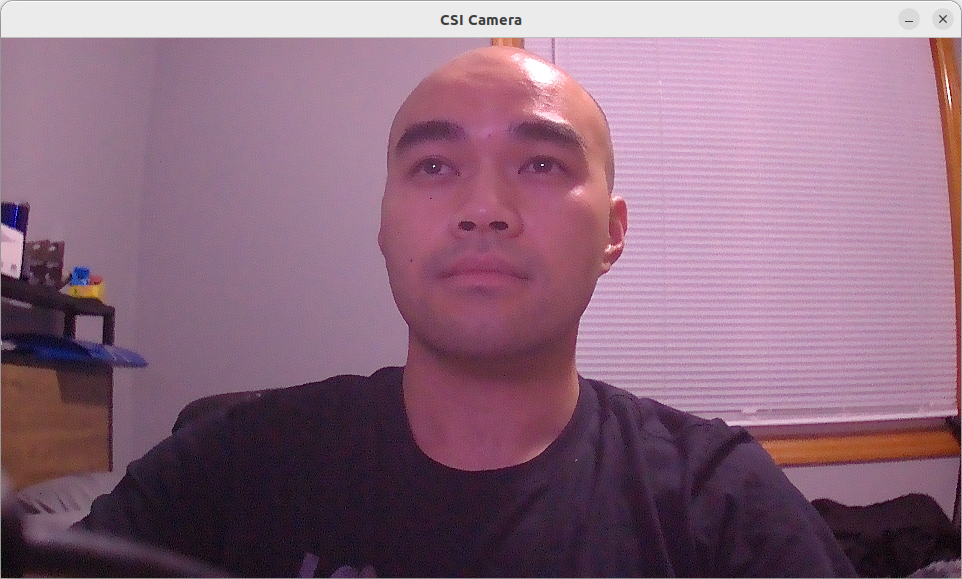
\includegraphics[width=\linewidth]{pics/light_normal.png}
                \caption*{(a) Has light without NIR}
            \end{minipage}\hfill
            \begin{minipage}{0.32\textwidth}
                \centering
                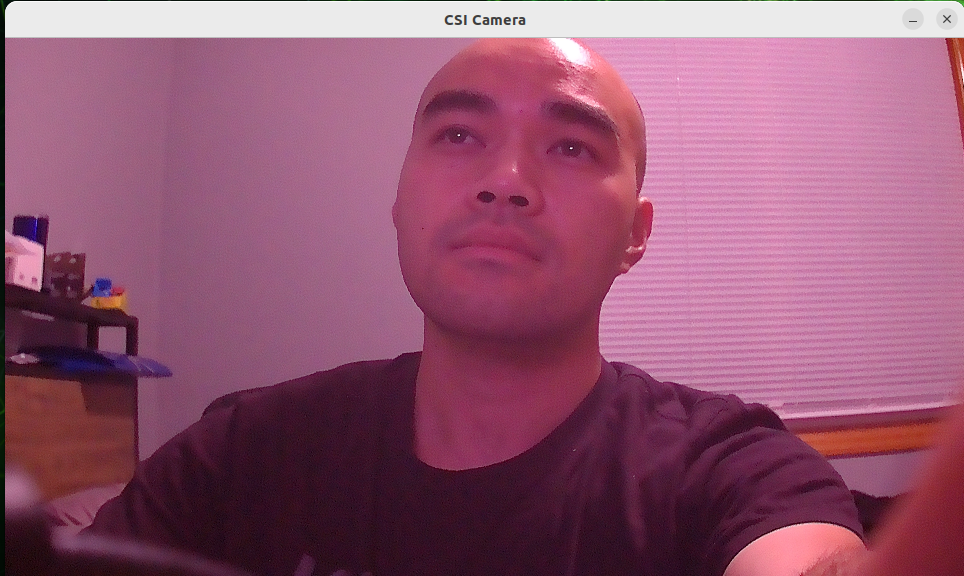
\includegraphics[width=\linewidth]{pics/light_IRCUT.png}
                \caption*{(b) Has light with NIR}
            \end{minipage}\hfill
            \begin{minipage}{0.32\textwidth}
            \centering
            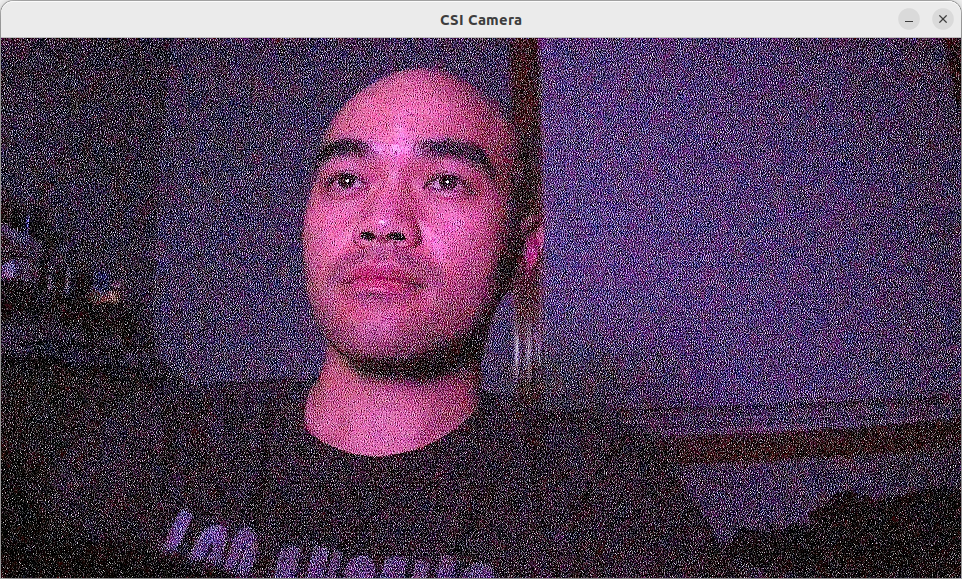
\includegraphics[width=\linewidth]{pics/dark.png}
            \caption*{(c) No light with NIR}
            \end{minipage}
    
            \caption{Live image comparison between three mode from ArduCam.}
            \label{fig:three_mode_image}
        \end{figure}

        
        
        

\newpage

%%%%%%%%%%%%%%%%%%%%%%%%%%%%%%%%%%%%%%%%%%%%%%%%%%%%%%%%%%%%%%%%%%%%%%%%%%%%%%%%%%%%%%%%%%%%%%%%%%%%%%%%%%%%%%%%%%%%%%
\section{Encountered Issue}
\label{sec:issue}
\vspace{10.5cm}


    \subsection{Chromium and Firefox not working}
    \label{subsec:issue_chromium_firefox}

    
    \begin{description}
        \item[Symptoms:] After installed and booted up Jetson Orin nano with Jetpack, and installed Chromium or Firefox, they cannot be opened. Happened after finishing step \ref{subsubsec:flashing} and boot up.
        \item[Issue:] there is an issue with current version of snap. Rolling back snap/snapd version and hold for automatic update solve issue for now (using a older version like this is not recommended, a better solution is preffered).
        \item[Solution:] Command to fix.
        
        \begin{lstlisting}[style=bashstyle]
$ snap download snapd --revision=24724
$ sudo snap ack snapd_24724.assert
$ sudo snap install snapd_24724.snap
$ sudo sudo snap refresh --hold snapd
        \end{lstlisting}

        \item[Reference:] Link from Nvidia forum - {\footnotesize \url{https://forums.developer.nvidia.com/t/neither-chromium-nor-firefox-work-with-my-jetson-orin-nano/338669}}

    \end{description}

    \subsection{Camera is not detected after connecting}
    \label{subsec:camera_not_detected}

    \begin{description}
        \item[Symptoms:] After connecting camera to Jetson Orin Nano by 22 pins FFC cable and try a camera app like \textbf{\emph{cheese}} or try simple camera testing script as mentioned in step \ref{} did not work. An error pointed to that camera is not detected. 
        
        \item[Issue:] By default the system and Jetpack seems to recognize IMX219. So, by connecting other type of camera, the system will not automatically detect it. the  
        \item[Solution:] use jetson-IO utility and enable IMX477. On terminal run:
            
        \begin{lstlisting}[style=bashstyle]
$ sudo /opt/nvidia/jetson-io/jetson-io.py
        \end{lstlisting}
    
        Then choose options as follow: \textbf{\emph{Configure Jetson 24pin CSI Connector}} -> \textbf{\emph{Configure for compatible hardware}} -> \textbf{\emph{Camera IMX477-A and IMX219-C}} then follow through the rest and reboot.
        
        \item[Reference:] Similar approach from Nvidia forum. Basically the same procedure as what he tried, but he has another issue which is connect cable the wrong way - {\footnotesize \url{https://forums.developer.nvidia.com/t/imx477-not-detected-by-third-party-carrier-boards-for-jetson-orin-nx-8gb/281710}}

    \end{description}










\addtocounter{section}{14}
\addcontentsline{toc}{section}{\protect\numberline{\thesection}~~~ References}
%%%%%%%%%%%%%%%%%%%%%%%%%%%%%%%%%%%%%%%%%%%%%%%%%%%%%%%%%%%%%%%%%%
\end{document}